%% ===========================================================================
%% figures-draft.tex — DIAGRAM WORKBENCH, NOT A SUBMISSION
%%
%% Every figure the NSysS paper might use, drawn at full size with no page
%% limit, so a diagram can be designed here and then pasted into main.tex.
%%
%% HOW TO USE
%%   1. Compile:  latexmk -pdf figures-draft.tex
%%   2. Pick a figure, copy the tikzpicture between its BEGIN/END markers.
%%   3. Paste into main.tex inside \begin{figure}[t] ... \end{figure}
%%      (or figure* for a two-column-wide float).
%%   4. Shrink to column width: every figure here declares \FigScale. In the
%%      paper, wrap the picture in \resizebox{\columnwidth}{!}{...} or set
%%      [scale=0.8] on the tikzpicture, and drop font sizes one step.
%%
%% The colour palette and the tikz libraries below are IDENTICAL to main.tex.
%% If you change one, change both.
%% ===========================================================================
\documentclass[11pt]{article}
\usepackage[a3paper,margin=18mm,landscape]{geometry}
\usepackage{amsmath}
\usepackage{tikz}
\usepackage{booktabs}
\usepackage{pgfplots}
\pgfplotsset{compat=1.18}
\usetikzlibrary{arrows.meta,positioning,fit,backgrounds,calc,shapes.geometric,
                decorations.pathreplacing,patterns}

%% ── palette (same as main.tex) ─────────────────────────────────────────────
\definecolor{jbInk}{HTML}{1F2933}
\definecolor{jbBlue}{HTML}{2C6E9B}
\definecolor{jbTeal}{HTML}{3F8F7A}
\definecolor{jbAmber}{HTML}{C6873B}
\definecolor{jbRose}{HTML}{A8465F}
\definecolor{jbMist}{HTML}{DDE3E8}

%% ── shared styles ──────────────────────────────────────────────────────────
\tikzset{
  box/.style       ={draw=jbInk,line width=0.4pt,rounded corners=1pt,
                     inner xsep=3pt,inner ysep=2.5pt,font=\scriptsize},
  nodebox/.style   ={box,fill=white,minimum width=13mm,minimum height=6mm},
  islandA/.style   ={box,fill=jbTeal!14},
  islandB/.style   ={box,fill=jbBlue!12},
  bridgebox/.style ={box,fill=jbAmber!22,line width=0.7pt},
  store/.style     ={box,fill=jbMist,minimum width=13mm,minimum height=5.5mm},
  pstep/.style     ={draw=jbInk,line width=0.3pt,minimum height=5mm,
                     minimum width=6.6mm,inner sep=1pt,font=\tiny,fill=white},
  nowrite/.style   ={pstep,fill=jbTeal!16},
  atomic/.style    ={pstep,fill=jbRose!20},
  emit/.style      ={pstep,fill=jbAmber!20},
  flow/.style      ={-{Stealth[length=1.5mm]},jbInk,line width=0.45pt},
  flowdash/.style  ={flow,dashed},
  cut/.style       ={jbRose,line width=0.9pt},
  lbl/.style       ={font=\scriptsize,text=jbInk},
  slbl/.style      ={font=\tiny,text=jbInk},
  ilbl/.style      ={font=\scriptsize\itshape,text=jbInk},
  %% sequence-diagram styles
  actor/.style     ={box,fill=jbMist,minimum width=17mm,minimum height=5.5mm,
                     font=\scriptsize\bfseries},
  life/.style      ={jbInk!40,line width=0.35pt,dash pattern=on 1pt off 1.2pt},
  msg/.style       ={-{Stealth[length=1.4mm]},jbInk,line width=0.45pt},
  ret/.style       ={-{Stealth[length=1.4mm]},jbInk!65,line width=0.4pt,dashed},
  self/.style      ={-{Stealth[length=1.4mm]},jbInk,line width=0.45pt},
  mlbl/.style      ={font=\tiny,text=jbInk,inner sep=1.2pt,fill=white},
  actbar/.style    ={draw=jbInk,fill=jbTeal!25,line width=0.3pt,minimum width=1.6mm},
  note/.style      ={box,fill=jbAmber!14,font=\tiny,align=left,inner sep=2.5pt},
}

\newcommand{\figtitle}[2]{%
  \bigskip\noindent{\large\bfseries #1}\\[2pt]
  {\small\itshape #2}\par\medskip}

\begin{document}
\begin{center}
{\LARGE\bfseries Diagram workbench}\\[4pt]
{\itshape Figures for the NSysS submission, drawn full size. Nothing here is page-limited.}
\end{center}
\medskip
\hrule
\bigskip

%% ===========================================================================
\figtitle{Figure A — Resilience ladder, reframed to L0--L3}
{Replaces the L0--L5 ladder in main.tex. The mesh and radio rungs are gone: this
system is a forum that survives blocking and blackout over IP, and off-grid
transport is explicitly not claimed. The right column names who cuts each rung,
which is what makes the ladder a threat statement and not a feature list.}

%% ---- BEGIN FIGURE A -------------------------------------------------------
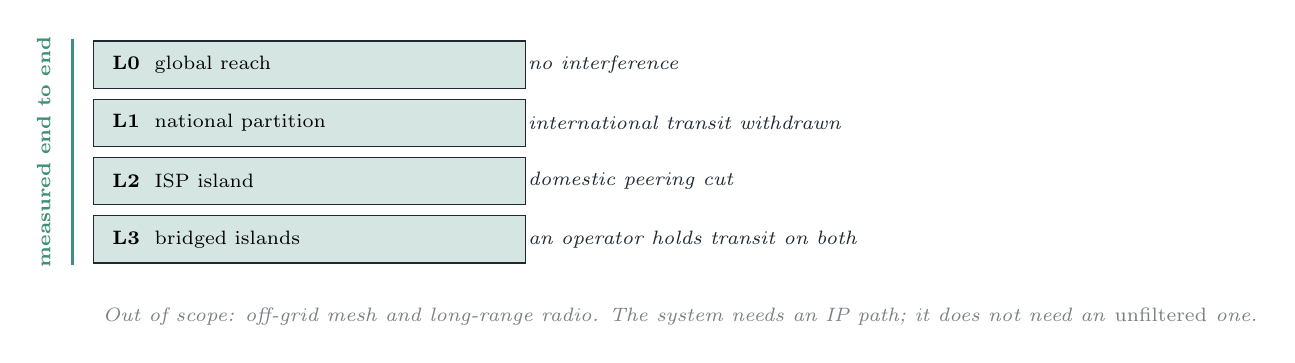
\begin{tikzpicture}[
  font=\scriptsize,
  rung/.style={draw=jbInk,line width=0.4pt,minimum height=6mm,inner xsep=4pt,anchor=west},
  ours/.style={rung,fill=jbTeal!22},
]
\def\W{52mm}
\foreach \i/\name/\what/\who in {
  0/L0/global reach/{no interference},
  1/L1/national partition/{international transit withdrawn},
  2/L2/ISP island/{domestic peering cut},
  3/L3/bridged islands/{an operator holds transit on both}}
{
  \node[ours,minimum width=\W] (r\i) at (0,{-\i*7.4mm})
    {\makebox[\W][l]{\ \textbf{\name}\ \ \what}};
  \node[ilbl,anchor=west] at (54mm,{-\i*7.4mm}) {\who};
}
\draw[jbTeal,line width=1.2pt] (-2.6mm,3.2mm) -- (-2.6mm,-25.5mm);
\node[rotate=90,anchor=south,font=\scriptsize\bfseries,text=jbTeal]
  at (-4.2mm,-11.1mm) {measured end to end};
\node[ilbl,anchor=west,text=jbInk!60] at (0,-32mm)
  {Out of scope: off-grid mesh and long-range radio. The system needs an IP path; it does not need
   an \emph{unfiltered} one.};
\end{tikzpicture}
%% ---- END FIGURE A ---------------------------------------------------------

\clearpage
%% ===========================================================================
\figtitle{Figure B — One write path, and where an envelope goes}
{The architectural claim in one picture: a single write endpoint, one pipeline,
and three consumers of the same accepted envelope (projection, witness log,
outbox). Clients never speak the federation protocol.}

%% ---- BEGIN FIGURE B -------------------------------------------------------
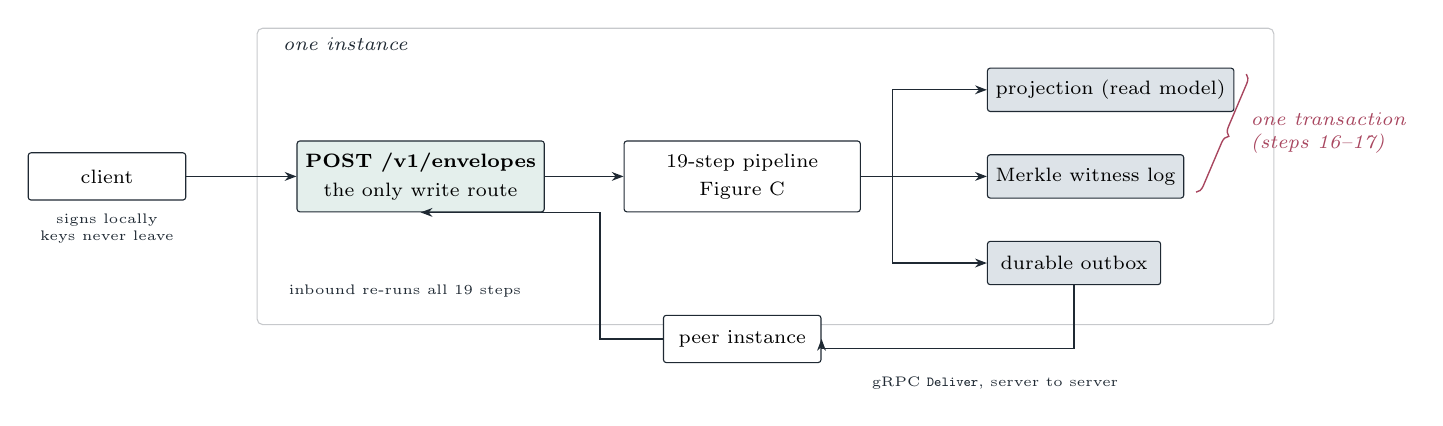
\begin{tikzpicture}[font=\scriptsize]
% client
\node[nodebox,minimum width=20mm] (client) at (0,0) {client};
\node[slbl,below=0.5mm of client,align=center] {signs locally\\keys never leave};

% ingress
\node[box,fill=jbTeal!14,minimum width=26mm,minimum height=9mm,right=14mm of client]
  (ingress) {\shortstack{\textbf{POST /v1/envelopes}\\[1pt]\scriptsize the only write route}};

% pipeline
\node[box,fill=white,minimum width=30mm,minimum height=9mm,right=10mm of ingress]
  (pipe) {\shortstack{19-step pipeline\\[1pt]\scriptsize Figure C}};

% outputs
\node[store,minimum width=22mm,right=16mm of pipe,yshift=11mm]  (proj)  {projection (read model)};
\node[store,minimum width=22mm,right=16mm of pipe]              (log)   {Merkle witness log};
\node[store,minimum width=22mm,right=16mm of pipe,yshift=-11mm] (outbox){durable outbox};

\draw[flow] (client) -- (ingress);
\draw[flow] (ingress) -- (pipe);
\draw[flow] (pipe.east) -- ++(4mm,0) |- (proj.west);
\draw[flow] (pipe.east) -- (log.west);
\draw[flow] (pipe.east) -- ++(4mm,0) |- (outbox.west);

% atomicity brace
\draw[decorate,decoration={brace,amplitude=3pt},jbRose,line width=0.5pt]
  ($(proj.east)+(1.5mm,2mm)$) -- ($(log.east)+(1.5mm,-2mm)$);
\node[ilbl,text=jbRose,anchor=west,align=left] at ($(proj.east)!0.5!(log.east)+(4mm,0)$)
  {one transaction\\(steps 16--17)};

% federation out
\node[nodebox,minimum width=20mm,below=13mm of pipe] (peer) {peer instance};
\draw[flow] (outbox.south) |- ++(0,-8mm) -| (peer.east);
\node[slbl,align=center] at ($(outbox.south)!0.5!(peer.east)+(6mm,-9mm)$)
  {gRPC \texttt{Deliver}, server to server};
\draw[flow] (peer.west) -- ++(-8mm,0) |- (ingress.south);
\node[slbl,align=center,anchor=north] at ($(ingress.south)+(-2mm,-8mm)$)
  {inbound re-runs all 19 steps};

\begin{scope}[on background layer]
\node[draw=jbInk!25,line width=0.4pt,rounded corners=2pt,inner sep=5mm,
      fit=(ingress)(pipe)(proj)(outbox)] (inst) {};
\end{scope}
\node[ilbl,anchor=north west] at (inst.north west) {\ \ one instance};
\end{tikzpicture}
%% ---- END FIGURE B ---------------------------------------------------------

\clearpage
%% ===========================================================================
\figtitle{Figure C — The nineteen-step validation pipeline}
{The paper names this pipeline a dozen times and never shows it. Two orderings
carry the argument and both are visible here: nothing before step 13 touches the
database (so an invalid flood cannot amplify into writes), and 16--17 commit
together (so nothing can be visible in a projection while missing from the log).}

%% ---- BEGIN FIGURE C -------------------------------------------------------
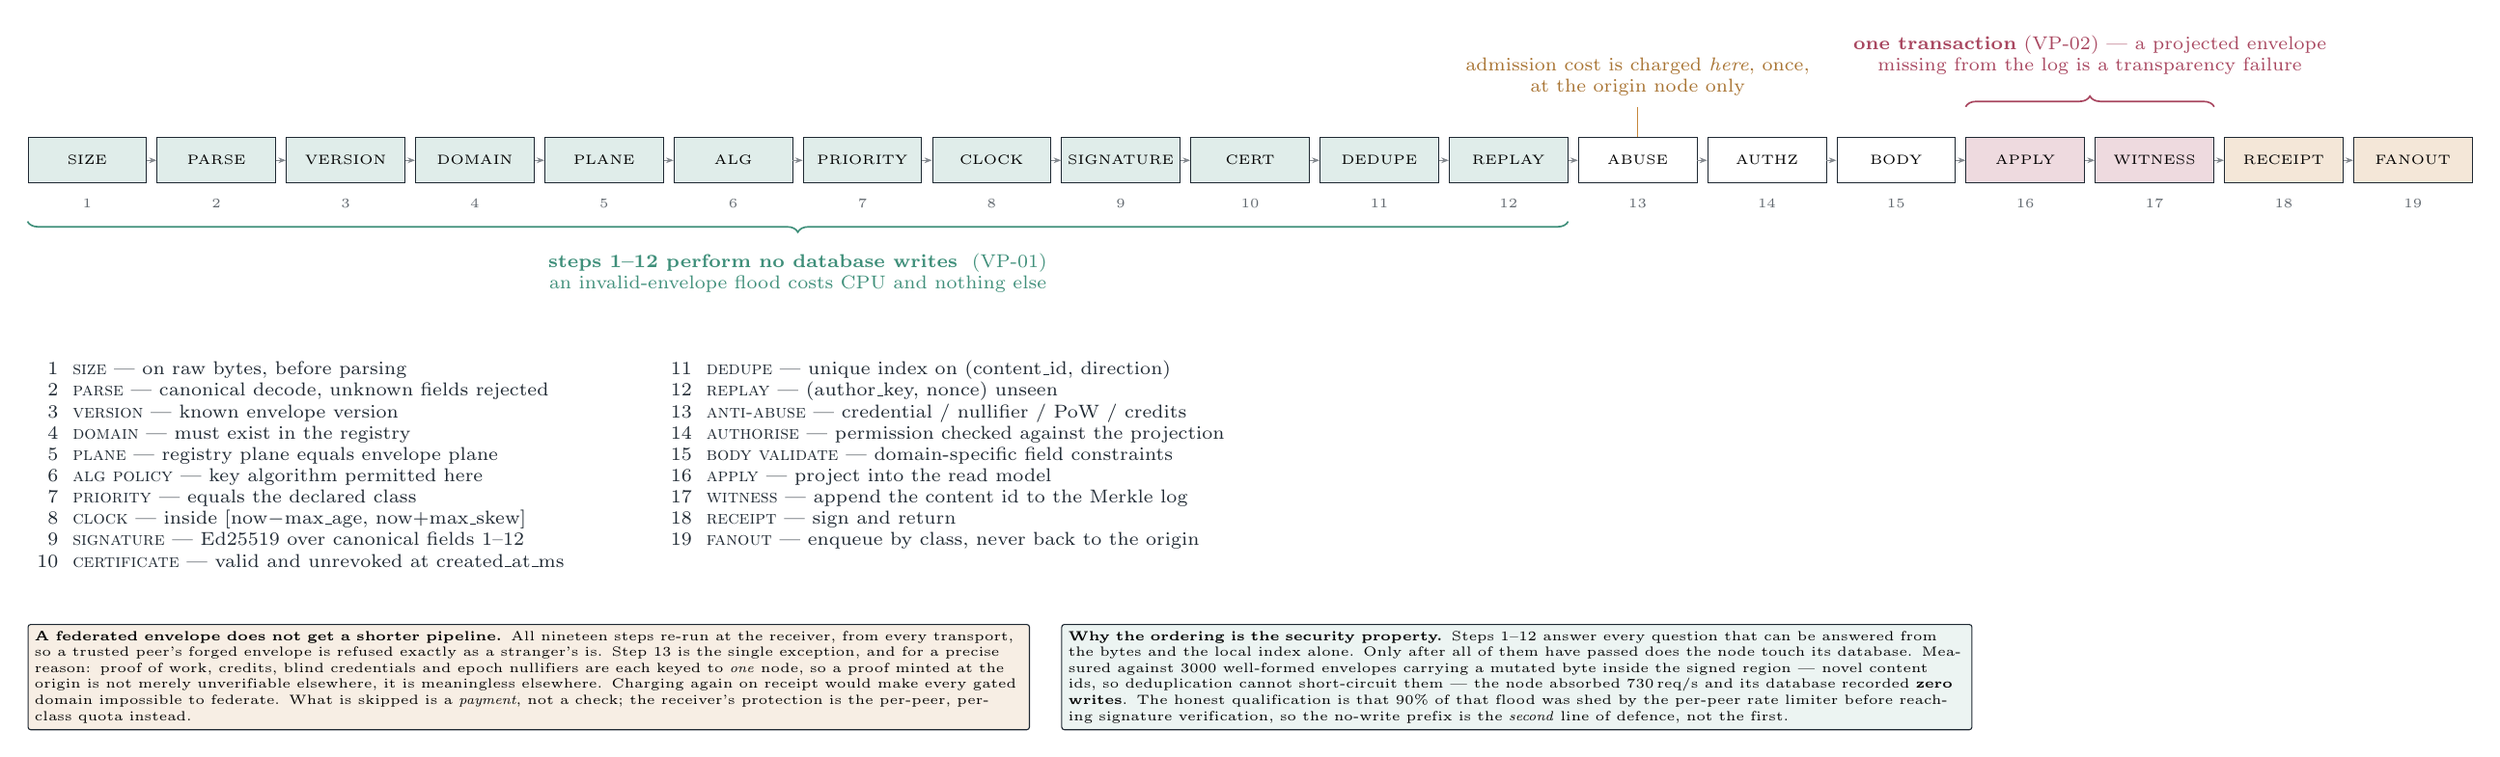
\begin{tikzpicture}[font=\scriptsize]
\def\dx{17mm}
\foreach \i/\name/\sty in {
   1/SIZE/nowrite,      2/PARSE/nowrite,     3/VERSION/nowrite,  4/DOMAIN/nowrite,
   5/PLANE/nowrite,     6/ALG/nowrite,       7/PRIORITY/nowrite, 8/CLOCK/nowrite,
   9/SIGNATURE/nowrite,10/CERT/nowrite,     11/DEDUPE/nowrite,  12/REPLAY/nowrite,
  13/ABUSE/pstep,      14/AUTHZ/pstep,      15/BODY/pstep,
  16/APPLY/atomic,     17/WITNESS/atomic,
  18/RECEIPT/emit,     19/FANOUT/emit}
{
  \node[\sty,minimum width=15.6mm,minimum height=6mm] (s\i) at ({(\i-1)*\dx},0) {\name};
  \node[font=\tiny,text=jbInk!70,below=0.8mm of s\i] {\i};
}
\foreach \i in {1,...,18}{
  \pgfmathtruncatemacro{\j}{\i+1}
  \draw[-{Stealth[length=1mm]},jbInk!55,line width=0.3pt] (s\i.east) -- (s\j.west);
}

% no-write bracket, below
\draw[decorate,decoration={brace,amplitude=4pt,mirror},jbTeal,line width=0.6pt]
  ($(s1.south west)+(0,-5mm)$) -- ($(s12.south east)+(0,-5mm)$);
\node[lbl,text=jbTeal,anchor=north,align=center]
  at ($(s1.south west)!0.5!(s12.south east)+(0,-8mm)$)
  {\textbf{steps 1--12 perform no database writes} \ (VP-01)\\
   an invalid-envelope flood costs CPU and nothing else};

% cost-charged marker on 13, drawn above so it clears the no-write caption
\draw[jbAmber,line width=0.5pt] (s13.north) -- ($(s13.north)+(0,4mm)$);
\node[lbl,text=jbAmber!85!black,anchor=south,align=center] at ($(s13.north)+(0,4.2mm)$)
  {admission cost is charged \emph{here}, once,\\at the origin node only};

% atomic bracket, above
\draw[decorate,decoration={brace,amplitude=4pt},jbRose,line width=0.6pt]
  ($(s16.north west)+(0,4mm)$) -- ($(s17.north east)+(0,4mm)$);
\node[lbl,text=jbRose,anchor=south,align=center]
  at ($(s16.north west)!0.5!(s17.north east)+(0,7mm)$)
  {\textbf{one transaction} (VP-02) --- a projected envelope\\missing from the log is a transparency failure};

% legend
\node[anchor=north west,align=left,font=\scriptsize,text=jbInk]
  at ($(s1.south west)+(0,-22mm)$)
{%
\begin{tabular}{@{}r@{\ \ }l@{\hspace{14mm}}r@{\ \ }l@{}}
 1 & \textsc{size} --- on raw bytes, before parsing        &11 & \textsc{dedupe} --- unique index on (content\_id, direction)\\
 2 & \textsc{parse} --- canonical decode, unknown fields rejected &12 & \textsc{replay} --- (author\_key, nonce) unseen\\
 3 & \textsc{version} --- known envelope version           &13 & \textsc{anti-abuse} --- credential / nullifier / PoW / credits\\
 4 & \textsc{domain} --- must exist in the registry        &14 & \textsc{authorise} --- permission checked against the projection\\
 5 & \textsc{plane} --- registry plane equals envelope plane&15 & \textsc{body validate} --- domain-specific field constraints\\
 6 & \textsc{alg policy} --- key algorithm permitted here  &16 & \textsc{apply} --- project into the read model\\
 7 & \textsc{priority} --- equals the declared class       &17 & \textsc{witness} --- append the content id to the Merkle log\\
 8 & \textsc{clock} --- inside [now$-$max\_age, now$+$max\_skew] &18 & \textsc{receipt} --- sign and return\\
 9 & \textsc{signature} --- Ed25519 over canonical fields 1--12 &19 & \textsc{fanout} --- enqueue by class, never back to the origin\\
10 & \textsc{certificate} --- valid and unrevoked at created\_at\_ms & & \\
\end{tabular}};

\node[note,anchor=north west,text width=130mm] at ($(s1.south west)+(0,-58mm)$)
{\textbf{A federated envelope does not get a shorter pipeline.} All nineteen steps re-run at the
receiver, from every transport, so a trusted peer's forged envelope is refused exactly as a
stranger's is. Step~13 is the single exception, and for a precise reason: proof of work, credits,
blind credentials and epoch nullifiers are each keyed to \emph{one} node, so a proof minted at the
origin is not merely unverifiable elsewhere, it is meaningless elsewhere. Charging again on receipt
would make every gated domain impossible to federate. What is skipped is a \emph{payment}, not a
check; the receiver's protection is the per-peer, per-class quota instead.};

\node[note,anchor=north west,text width=118mm,fill=jbTeal!10] at ($(s1.south west)+(136mm,-58mm)$)
{\textbf{Why the ordering is the security property.} Steps 1--12 answer every question that can be
answered from the bytes and the local index alone. Only after all of them have passed does the node
touch its database. Measured against 3000 well-formed envelopes carrying a mutated byte inside the
signed region --- novel content ids, so deduplication cannot short-circuit them --- the node absorbed
730\,req/s and its database recorded \textbf{zero writes}. The honest qualification is that 90\% of
that flood was shed by the per-peer rate limiter before reaching signature verification, so the
no-write prefix is the \emph{second} line of defence, not the first.};
\end{tikzpicture}
%% ---- END FIGURE C ---------------------------------------------------------

\clearpage
%% ===========================================================================
\figtitle{Figure D — ISP bridging: topology, source binding and quota}
{The L3 mechanism at full detail. Two islands on separate ASNs, the exchange
between them cut, and one node holding transit on both. The bridge binds each
outbound federation connection to the source address of the matching uplink,
which is what \texttt{/proc/net/tcp} is read to confirm.}

%% ---- BEGIN FIGURE D -------------------------------------------------------
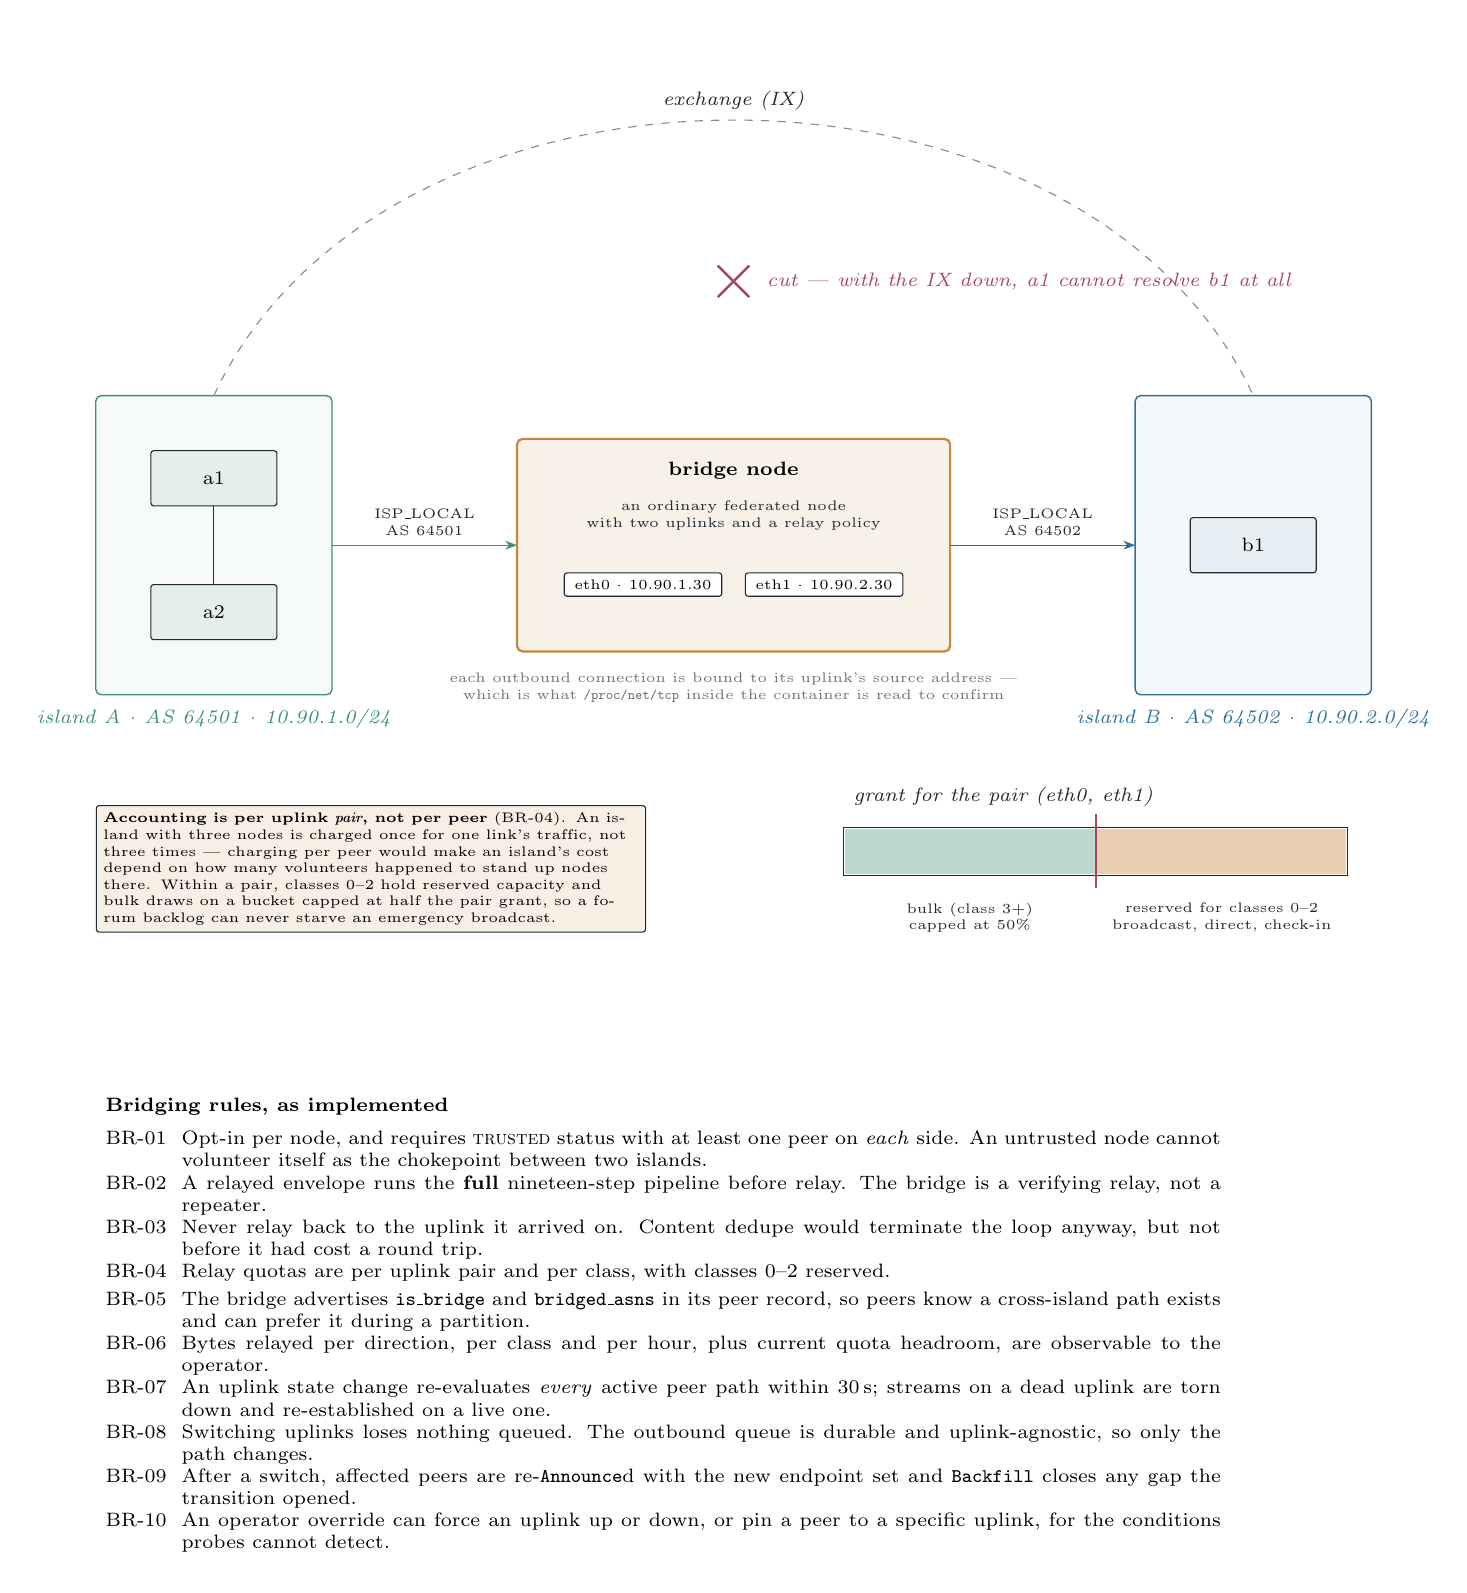
\begin{tikzpicture}[font=\scriptsize]
% ── island A ───────────────────────────────────────────────────────────────
\draw[draw=jbTeal,line width=0.5pt,rounded corners=2pt,fill=jbTeal!5]
  (-1.5,-1.9) rectangle (1.5,1.9);
\node[ilbl,text=jbTeal,anchor=north] at (0,-1.95)
  {island A \textperiodcentered\ AS 64501 \textperiodcentered\ 10.90.1.0/24};
\node[islandA,minimum width=16mm,minimum height=7mm] (a1) at (0,0.85)  {a1};
\node[islandA,minimum width=16mm,minimum height=7mm] (a2) at (0,-0.85) {a2};
\draw[jbInk,line width=0.4pt] (a1) -- (a2);

% ── bridge ─────────────────────────────────────────────────────────────────
\draw[draw=jbAmber,line width=0.8pt,rounded corners=2pt,fill=jbAmber!12]
  (3.85,-1.35) rectangle (9.35,1.35);
\node[font=\scriptsize\bfseries] at (6.6,0.95) {bridge node};
\node[slbl,align=center] at (6.6,0.38)
  {an ordinary federated node\\with two uplinks and a relay policy};
\node[box,fill=white,font=\tiny,minimum width=20mm] (up1) at (5.45,-0.5) {eth0 \textperiodcentered\ 10.90.1.30};
\node[box,fill=white,font=\tiny,minimum width=20mm] (up2) at (7.75,-0.5) {eth1 \textperiodcentered\ 10.90.2.30};
\node[slbl,text=jbInk!65,anchor=north,align=center] at (6.6,-1.5)
  {each outbound connection is bound to its uplink's source address ---\\
   which is what \texttt{/proc/net/tcp} inside the container is read to confirm};

% ── island B ───────────────────────────────────────────────────────────────
\draw[draw=jbBlue,line width=0.5pt,rounded corners=2pt,fill=jbBlue!5]
  (11.7,-1.9) rectangle (14.7,1.9);
\node[ilbl,text=jbBlue,anchor=north] at (13.2,-1.95)
  {island B \textperiodcentered\ AS 64502 \textperiodcentered\ 10.90.2.0/24};
\node[islandB,minimum width=16mm,minimum height=7mm] (b1) at (13.2,0) {b1};

\draw[flow,jbTeal] (1.5,0) -- node[slbl,above,align=center]{ISP\_LOCAL\\AS 64501} (3.85,0);
\draw[flow,jbBlue] (9.35,0) -- node[slbl,above,align=center]{ISP\_LOCAL\\AS 64502} (11.7,0);

% ── severed exchange ───────────────────────────────────────────────────────
\draw[dashed,jbInk!55] (0,1.9) to[out=65,in=115] node[pos=0.5,above,ilbl]{exchange (IX)} (13.2,1.9);
\coordinate (x) at (6.6,3.35);
\draw[cut] ($(x)+(-2mm,-2mm)$) -- ($(x)+(2mm,2mm)$);
\draw[cut] ($(x)+(2mm,-2mm)$) -- ($(x)+(-2mm,2mm)$);
\node[ilbl,text=jbRose,anchor=west] at ($(x)+(3mm,0)$)
  {cut --- with the IX down, a1 cannot resolve b1 at all};

% ── quota model ────────────────────────────────────────────────────────────
\node[note,anchor=north west,text width=68mm] at (-1.5,-3.3)
{\textbf{Accounting is per uplink \emph{pair}, not per peer} (BR-04). An island with three nodes is
charged once for one link's traffic, not three times --- charging per peer would make an island's
cost depend on how many volunteers happened to stand up nodes there. Within a pair, classes 0--2
hold reserved capacity and bulk draws on a bucket capped at half the pair grant, so a forum backlog
can never starve an emergency broadcast.};

\begin{scope}[shift={(8.0,-4.2)}]
  \node[ilbl,anchor=west] at (0,1.0) {grant for the pair (eth0, eth1)};
  \draw[draw=jbInk,line width=0.4pt] (0,0) rectangle (6.4,0.62);
  \fill[jbTeal!35] (0.02,0.02) rectangle (3.2,0.6);
  \fill[jbAmber!40] (3.2,0.02) rectangle (6.38,0.6);
  \draw[jbRose,line width=0.8pt] (3.2,-0.16) -- (3.2,0.78);
  \node[slbl,anchor=north,align=center] at (1.6,-0.22) {bulk (class 3+)\\capped at 50\%};
  \node[slbl,anchor=north,align=center] at (4.8,-0.22) {reserved for classes 0--2\\broadcast, direct, check-in};
\end{scope}

% ── rules ──────────────────────────────────────────────────────────────────
\node[anchor=north west,align=left,font=\scriptsize] at (-1.5,-6.9)
{\textbf{Bridging rules, as implemented}\\[4pt]
\begin{tabular}{@{}l@{\ \ }p{132mm}@{}}
BR-01 & Opt-in per node, and requires \textsc{trusted} status with at least one peer on \emph{each} side. An untrusted node cannot volunteer itself as the chokepoint between two islands.\\[2pt]
BR-02 & A relayed envelope runs the \textbf{full} nineteen-step pipeline before relay. The bridge is a verifying relay, not a repeater.\\[2pt]
BR-03 & Never relay back to the uplink it arrived on. Content dedupe would terminate the loop anyway, but not before it had cost a round trip.\\[2pt]
BR-04 & Relay quotas are per uplink pair and per class, with classes 0--2 reserved.\\[2pt]
BR-05 & The bridge advertises \texttt{is\_bridge} and \texttt{bridged\_asns} in its peer record, so peers know a cross-island path exists and can prefer it during a partition.\\[2pt]
BR-06 & Bytes relayed per direction, per class and per hour, plus current quota headroom, are observable to the operator.\\[2pt]
BR-07 & An uplink state change re-evaluates \emph{every} active peer path within 30\,s; streams on a dead uplink are torn down and re-established on a live one.\\[2pt]
BR-08 & Switching uplinks loses nothing queued. The outbound queue is durable and uplink-agnostic, so only the path changes.\\[2pt]
BR-09 & After a switch, affected peers are re-\texttt{Announce}d with the new endpoint set and \texttt{Backfill} closes any gap the transition opened.\\[2pt]
BR-10 & An operator override can force an uplink up or down, or pin a peer to a specific uplink, for the conditions probes cannot detect.\\
\end{tabular}};
\end{tikzpicture}
%% ---- END FIGURE D ---------------------------------------------------------

\clearpage
%% ===========================================================================
\figtitle{Figure E — Sequence: publish once, federate to a peer}
{The ordinary path, with the two things reviewers ask about marked: the receipt
is returned before fanout, and the peer re-runs every validation step.}

%% ---- BEGIN FIGURE E -------------------------------------------------------
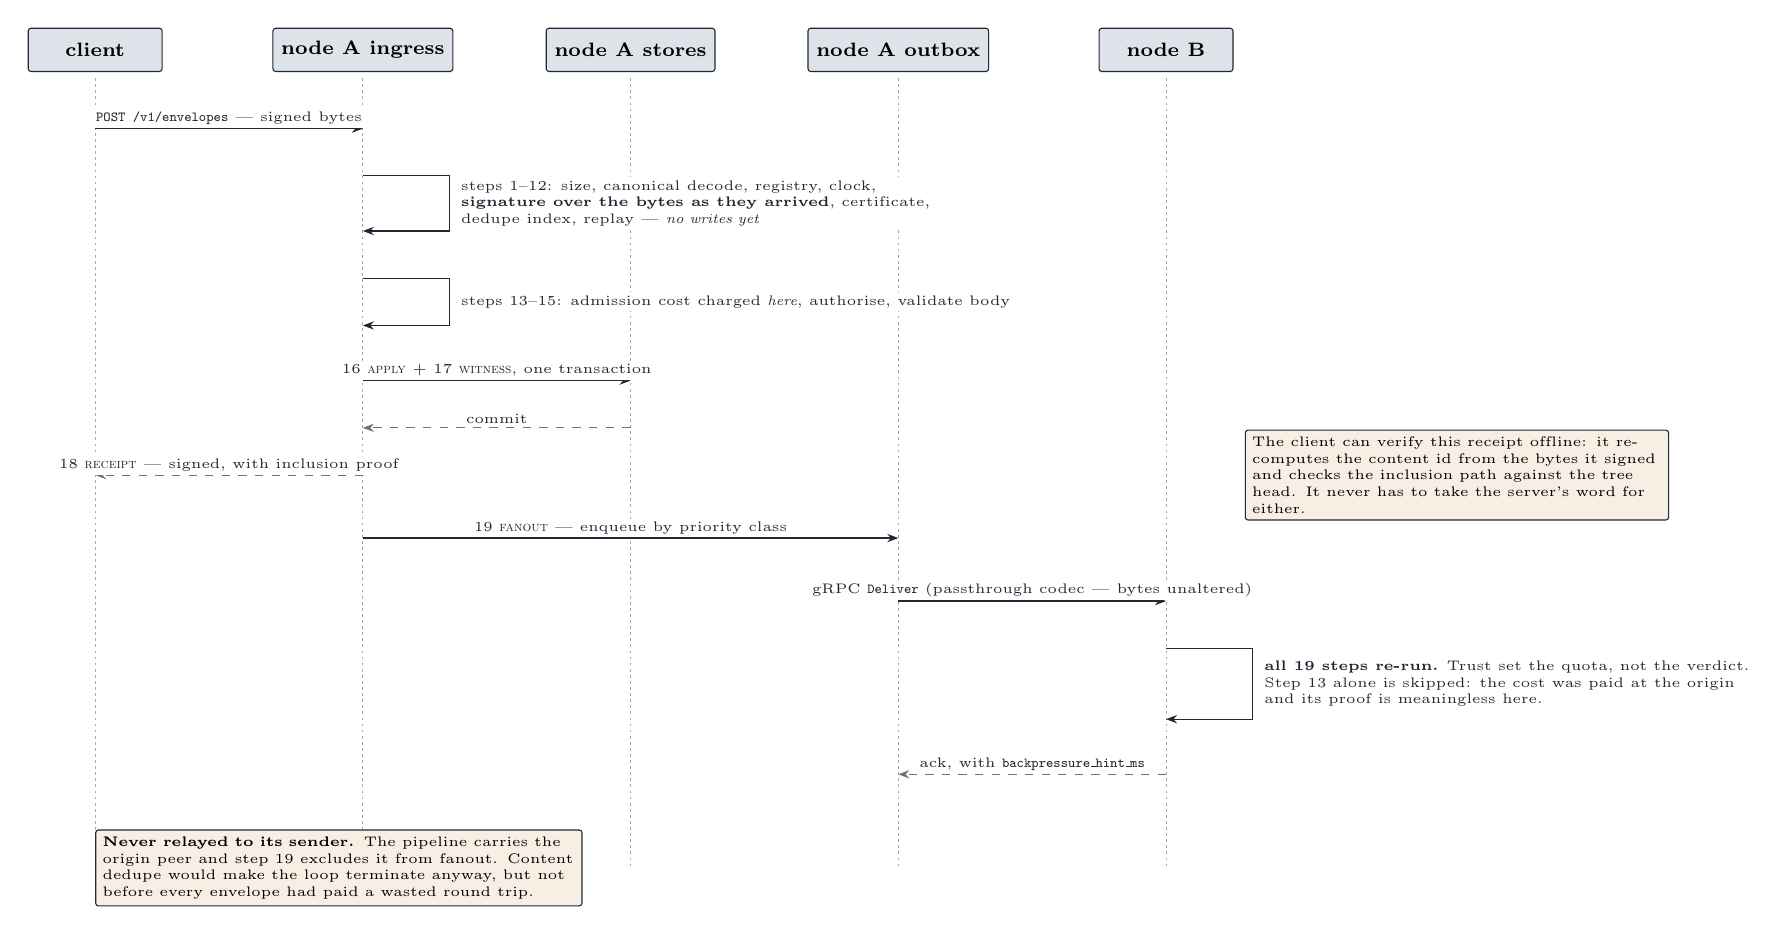
\begin{tikzpicture}[font=\scriptsize]
\def\H{-10.4}
\foreach \x/\n in {0/{client}, 3.4/{node A ingress}, 6.8/{node A stores}, 10.2/{node A outbox}, 13.6/{node B}}
  { \node[actor] (A\x) at (\x,0) {\n};
    \draw[life] (\x,-0.36) -- (\x,\H); }

\newcommand{\seqmsg}[4]{\draw[msg] (#1,#3) -- (#2,#3) node[mlbl,midway,above]{#4};}
\newcommand{\seqret}[4]{\draw[ret] (#1,#3) -- (#2,#3) node[mlbl,midway,above]{#4};}

\seqmsg{0}{3.4}{-1.0}{\texttt{POST /v1/envelopes} — signed bytes}
\draw[self] (3.4,-1.6) -- (4.5,-1.6) -- (4.5,-2.3) -- (3.4,-2.3);
\node[mlbl,anchor=west,align=left] at (4.6,-1.95)
  {steps 1--12: size, canonical decode, registry, clock,\\
   \textbf{signature over the bytes as they arrived}, certificate,\\
   dedupe index, replay — \emph{no writes yet}};
\draw[self] (3.4,-2.9) -- (4.5,-2.9) -- (4.5,-3.5) -- (3.4,-3.5);
\node[mlbl,anchor=west,align=left] at (4.6,-3.2)
  {steps 13--15: admission cost charged \emph{here}, authorise, validate body};

\seqmsg{3.4}{6.8}{-4.2}{16 \textsc{apply} + 17 \textsc{witness}, one transaction}
\seqret{6.8}{3.4}{-4.8}{commit}
\seqret{3.4}{0}{-5.4}{18 \textsc{receipt} — signed, with inclusion proof}
\node[note,anchor=west,text width=52mm] at (14.6,-5.4)
  {The client can verify this receipt offline: it recomputes the content id from the bytes it
   signed and checks the inclusion path against the tree head. It never has to take the server's
   word for either.};

\seqmsg{3.4}{10.2}{-6.2}{19 \textsc{fanout} — enqueue by priority class}
\seqmsg{10.2}{13.6}{-7.0}{gRPC \texttt{Deliver} (passthrough codec — bytes unaltered)}
\draw[self] (13.6,-7.6) -- (14.7,-7.6) -- (14.7,-8.5) -- (13.6,-8.5);
\node[mlbl,anchor=west,align=left] at (14.8,-8.05)
  {\textbf{all 19 steps re-run.} Trust set the quota, not the verdict.\\
   Step 13 alone is skipped: the cost was paid at the origin\\
   and its proof is meaningless here.};
\seqret{13.6}{10.2}{-9.2}{ack, with \texttt{backpressure\_hint\_ms}}
\node[note,anchor=north west,text width=60mm] at (0,-9.9)
  {\textbf{Never relayed to its sender.} The pipeline carries the origin peer and step 19 excludes it
   from fanout. Content dedupe would make the loop terminate anyway, but not before every envelope
   had paid a wasted round trip.};
\end{tikzpicture}
%% ---- END FIGURE E ---------------------------------------------------------

\clearpage
%% ===========================================================================
\figtitle{Figure F — Sequence: a crossing after the exchange is cut}
{Why a "crossing" is three envelopes and not one. A post that island B can
actually render needs the author's certificate and the community record first,
so the measured cost is the whole dependency chain — 0.5\,s, 1.2\,s, 2.1\,s.}

%% ---- BEGIN FIGURE F -------------------------------------------------------
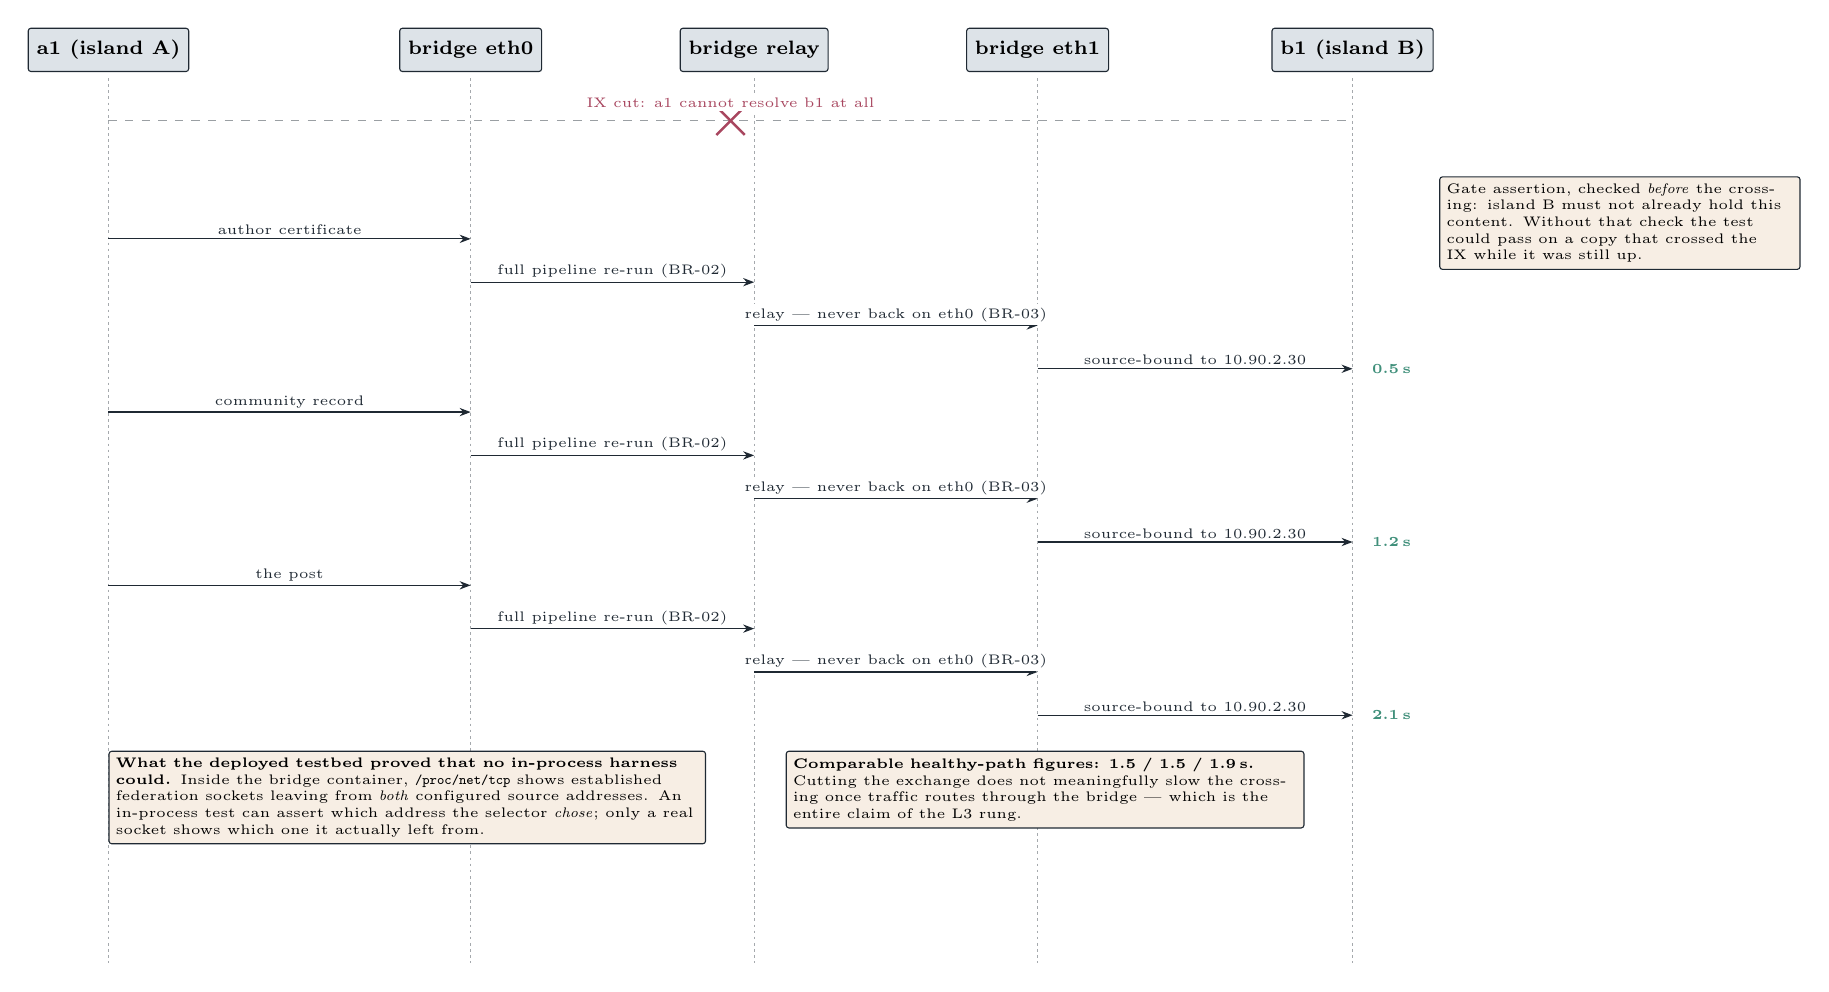
\begin{tikzpicture}[font=\scriptsize]
\def\H{-11.6}
\foreach \x/\n in {0/{a1 (island A)}, 4.6/{bridge eth0}, 8.2/{bridge relay}, 11.8/{bridge eth1}, 15.8/{b1 (island B)}}
  { \node[actor] (A\x) at (\x,0) {\n};
    \draw[life] (\x,-0.36) -- (\x,\H); }

\newcommand{\seqmsg}[4]{\draw[msg] (#1,#3) -- (#2,#3) node[mlbl,midway,above]{#4};}

% the cut
\draw[dashed,jbInk!45] (0,-0.9) -- (15.8,-0.9);
\coordinate (c) at (7.9,-0.9);
\draw[cut] ($(c)+(-1.8mm,-1.8mm)$) -- ($(c)+(1.8mm,1.8mm)$);
\draw[cut] ($(c)+(1.8mm,-1.8mm)$) -- ($(c)+(-1.8mm,1.8mm)$);
\node[mlbl,text=jbRose,anchor=south] at (7.9,-0.78) {IX cut: a1 cannot resolve b1 at all};

\node[note,anchor=west,text width=44mm] at (16.9,-2.2)
  {Gate assertion, checked \emph{before} the crossing: island B must not already hold this content.
   Without that check the test could pass on a copy that crossed the IX while it was still up.};

\foreach \k/\y/\what/\t in {1/-2.4/{author certificate}/{0.5\,s},
                           2/-4.6/{community record}/{1.2\,s},
                           3/-6.8/{the post}/{2.1\,s}}
{
  \seqmsg{0}{4.6}{\y}{\what}
  \draw[msg] (4.6,\y-0.55) -- (8.2,\y-0.55)
    node[mlbl,midway,above]{full pipeline re-run (BR-02)};
  \draw[msg] (8.2,\y-1.1) -- (11.8,\y-1.1)
    node[mlbl,midway,above]{relay — never back on eth0 (BR-03)};
  \draw[msg] (11.8,\y-1.65) -- (15.8,\y-1.65)
    node[mlbl,midway,above]{source-bound to 10.90.2.30};
  \node[mlbl,anchor=west,text=jbTeal] at (16.0,\y-1.65) {\textbf{\t}};
}

\node[note,anchor=north west,text width=74mm] at (0,-8.9)
  {\textbf{What the deployed testbed proved that no in-process harness could.} Inside the bridge
   container, \texttt{/proc/net/tcp} shows established federation sockets leaving from \emph{both}
   configured source addresses. An in-process test can assert which address the selector \emph{chose};
   only a real socket shows which one it actually left from.};
\node[note,anchor=north west,text width=64mm] at (8.6,-8.9)
  {\textbf{Comparable healthy-path figures: 1.5 / 1.5 / 1.9\,s.} Cutting the exchange does not
   meaningfully slow the crossing once traffic routes through the bridge — which is the entire
   claim of the L3 rung.};
\end{tikzpicture}
%% ---- END FIGURE F ---------------------------------------------------------

\clearpage
%% ===========================================================================
\figtitle{Figure G — Sequence: uplink failover without loss}
{BR-07 through BR-10 as one timeline. The property worth drawing is that the
queue is uplink-agnostic, so a switch changes the path and nothing else.}

%% ---- BEGIN FIGURE G -------------------------------------------------------
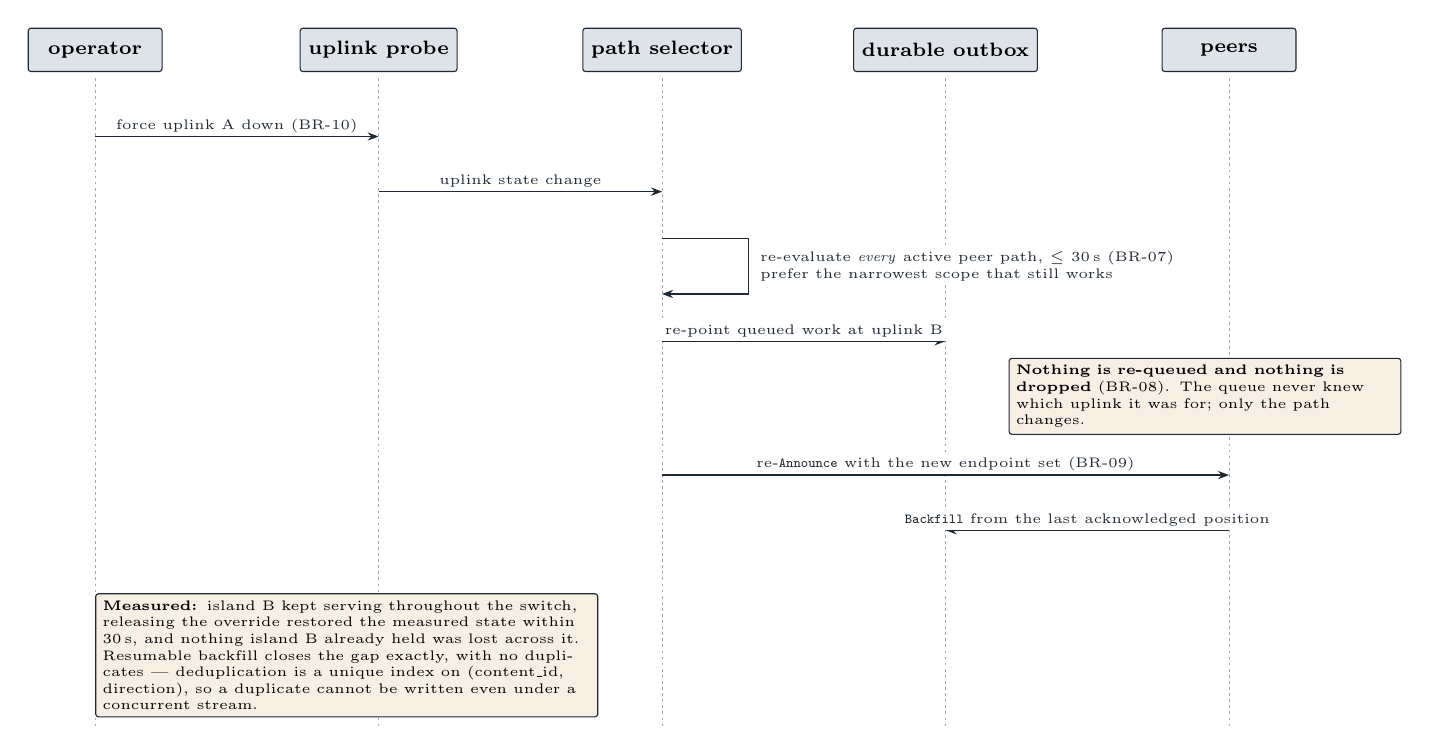
\begin{tikzpicture}[font=\scriptsize]
\def\H{-8.6}
\foreach \x/\n in {0/{operator}, 3.6/{uplink probe}, 7.2/{path selector}, 10.8/{durable outbox}, 14.4/{peers}}
  { \node[actor] (A\x) at (\x,0) {\n};
    \draw[life] (\x,-0.36) -- (\x,\H); }
\newcommand{\seqmsg}[4]{\draw[msg] (#1,#3) -- (#2,#3) node[mlbl,midway,above]{#4};}
\newcommand{\seqret}[4]{\draw[ret] (#1,#3) -- (#2,#3) node[mlbl,midway,above]{#4};}

\seqmsg{0}{3.6}{-1.1}{force uplink A down (BR-10)}
\seqmsg{3.6}{7.2}{-1.8}{uplink state change}
\draw[self] (7.2,-2.4) -- (8.3,-2.4) -- (8.3,-3.1) -- (7.2,-3.1);
\node[mlbl,anchor=west,align=left] at (8.4,-2.75)
  {re-evaluate \emph{every} active peer path, $\le$ 30\,s (BR-07)\\
   prefer the narrowest scope that still works};
\seqmsg{7.2}{10.8}{-3.7}{re-point queued work at uplink B}
\node[note,anchor=west,text width=48mm] at (11.6,-4.4)
  {\textbf{Nothing is re-queued and nothing is dropped} (BR-08). The queue never knew which uplink it
   was for; only the path changes.};
\seqmsg{7.2}{14.4}{-5.4}{re-\texttt{Announce} with the new endpoint set (BR-09)}
\seqmsg{14.4}{10.8}{-6.1}{\texttt{Backfill} from the last acknowledged position}
\node[note,anchor=north west,text width=62mm] at (0,-6.9)
  {\textbf{Measured:} island B kept serving throughout the switch, releasing the override restored the
   measured state within 30\,s, and nothing island B already held was lost across it. Resumable
   backfill closes the gap exactly, with no duplicates — deduplication is a unique index on
   (content\_id, direction), so a duplicate cannot be written even under a concurrent stream.};
\end{tikzpicture}
%% ---- END FIGURE G ---------------------------------------------------------

\clearpage
%% ===========================================================================
\figtitle{Figure H — Sequence: a stale tree head is not evidence of a fork}
{The defect and the fix in one diagram. Four code paths sample a peer's head and
nothing orders their arrival, so an older reading routinely lands after a fresher
one. Compared pairwise with no consistency proof, that reads as a log rollback.}

%% ---- BEGIN FIGURE H -------------------------------------------------------
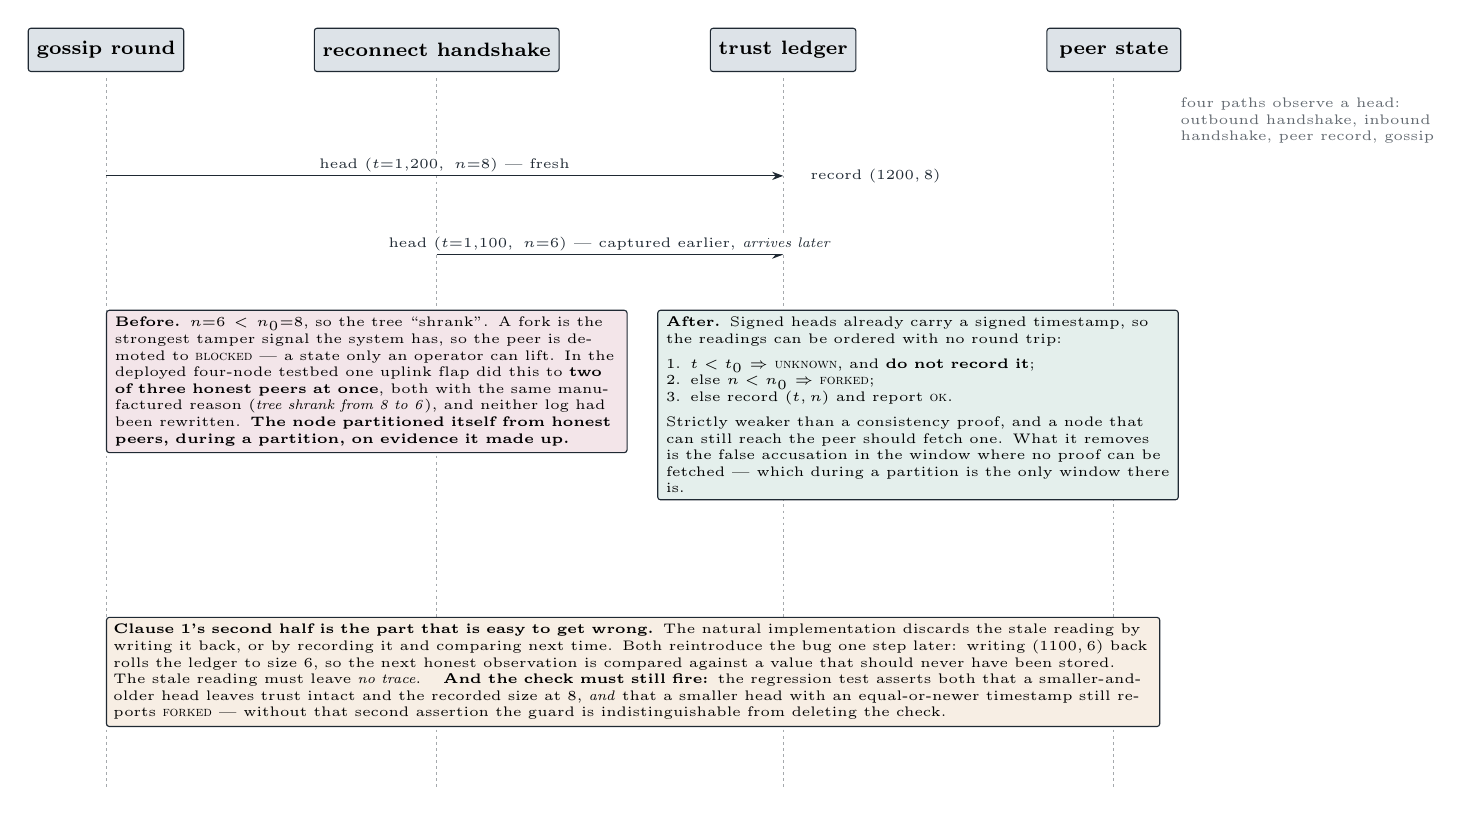
\begin{tikzpicture}[font=\scriptsize]
\def\H{-9.4}
\foreach \x/\n in {0/{gossip round}, 4.2/{reconnect handshake}, 8.6/{trust ledger}, 12.8/{peer state}}
  { \node[actor] (A\x) at (\x,0) {\n};
    \draw[life] (\x,-0.36) -- (\x,\H); }
\newcommand{\seqmsg}[4]{\draw[msg] (#1,#3) -- (#2,#3) node[mlbl,midway,above]{#4};}

\node[mlbl,anchor=west,align=left,text=jbInk!70] at (13.6,-0.9)
  {four paths observe a head:\\outbound handshake, inbound\\handshake, peer record, gossip};

\seqmsg{0}{8.6}{-1.6}{head $(t{=}1{,}200,\ n{=}8)$ — fresh}
\node[mlbl,anchor=west] at (8.9,-1.6) {record $(1200, 8)$};
\seqmsg{4.2}{8.6}{-2.6}{head $(t{=}1{,}100,\ n{=}6)$ — captured earlier, \emph{arrives later}}

% wrong branch
\node[box,fill=jbRose!14,anchor=north west,text width=64mm,align=left,font=\tiny]
  at (0,-3.3)
  {\textbf{Before.} $n{=}6 < n_0{=}8$, so the tree ``shrank''. A fork is the strongest tamper signal
   the system has, so the peer is demoted to \textsc{blocked} — a state only an operator can lift.
   In the deployed four-node testbed one uplink flap did this to \textbf{two of three honest peers at
   once}, both with the same manufactured reason (\emph{tree shrank from 8 to 6}), and neither log had
   been rewritten. \textbf{The node partitioned itself from honest peers, during a partition, on
   evidence it made up.}};

\node[box,fill=jbTeal!14,anchor=north west,text width=64mm,align=left,font=\tiny]
  at (7.0,-3.3)
  {\textbf{After.} Signed heads already carry a signed timestamp, so the readings can be ordered
   with no round trip:\\[3pt]
   1. $t < t_0$ $\Rightarrow$ \textsc{unknown}, and \textbf{do not record it};\\
   2. else $n < n_0$ $\Rightarrow$ \textsc{forked};\\
   3. else record $(t,n)$ and report \textsc{ok}.\\[3pt]
   Strictly weaker than a consistency proof, and a node that can still reach the peer should fetch
   one. What it removes is the false accusation in the window where no proof can be fetched — which
   during a partition is the only window there is.};

\node[note,anchor=north west,text width=132mm] at (0,-7.2)
  {\textbf{Clause 1's second half is the part that is easy to get wrong.} The natural implementation
   discards the stale reading by writing it back, or by recording it and comparing next time. Both
   reintroduce the bug one step later: writing $(1100,6)$ back rolls the ledger to size 6, so the next
   honest observation is compared against a value that should never have been stored. The stale
   reading must leave \emph{no trace}. \ \ \textbf{And the check must still fire:} the regression test
   asserts both that a smaller-and-older head leaves trust intact and the recorded size at 8,
   \emph{and} that a smaller head with an equal-or-newer timestamp still reports \textsc{forked} —
   without that second assertion the guard is indistinguishable from deleting the check.};
\end{tikzpicture}
%% ---- END FIGURE H ---------------------------------------------------------

\clearpage
%% ===========================================================================
\figtitle{Figure I — Peer admission: TOFU, vouching, and the one state an operator must lift}
{Why there is no admin allowlist: during a shutdown, volunteers stand up relay
nodes and cannot wait for manual approval. New peers are admitted immediately at
a low quota and earn reach.}

%% ---- BEGIN FIGURE I -------------------------------------------------------
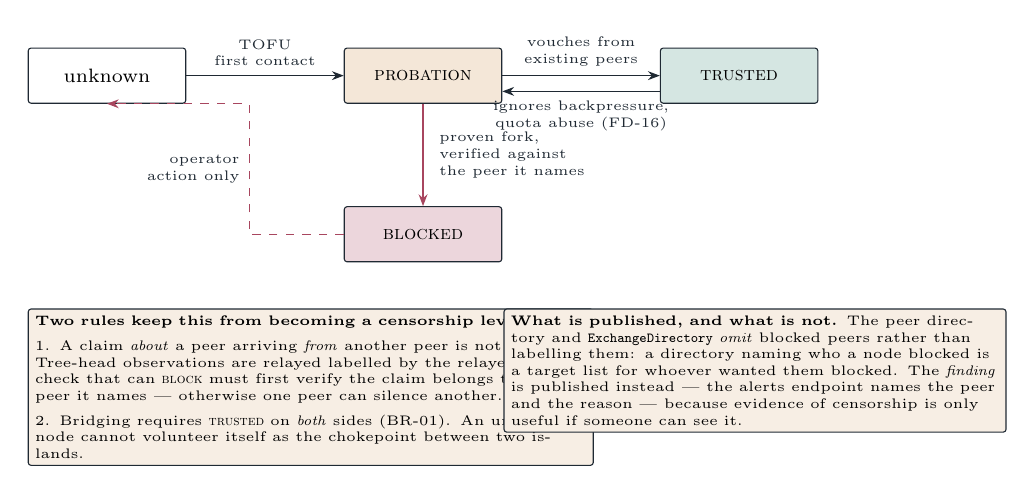
\begin{tikzpicture}[font=\scriptsize,node distance=15mm]
\node[box,fill=white,minimum width=20mm,minimum height=7mm] (unk) {unknown};
\node[box,fill=jbAmber!20,minimum width=20mm,minimum height=7mm,right=20mm of unk] (prob) {\textsc{probation}};
\node[box,fill=jbTeal!22,minimum width=20mm,minimum height=7mm,right=20mm of prob] (trust) {\textsc{trusted}};
\node[box,fill=jbRose!22,minimum width=20mm,minimum height=7mm,below=13mm of prob] (block) {\textsc{blocked}};

\draw[flow] (unk) -- node[slbl,above,align=center]{TOFU\\first contact} (prob);
\draw[flow] (prob) -- node[slbl,above,align=center]{vouches from\\existing peers} (trust);
\draw[flow] ([yshift=-2mm]trust.west) -- node[slbl,below,align=center]{ignores backpressure,\\quota abuse (FD-16)} ([yshift=-2mm]prob.east);
\draw[flow,jbRose] (prob) -- node[slbl,right,align=left]{\ proven fork,\\ \ verified against\\ \ the peer it names} (block);
\draw[flow,jbRose,dashed] (block.west) -- ++(-12mm,0) |- node[slbl,pos=0.25,left,align=right]{operator\\action only\ } (unk.south);

\node[note,anchor=north west,text width=70mm] at ($(unk.south west)+(0,-26mm)$)
{\textbf{Two rules keep this from becoming a censorship lever itself.}\\[3pt]
1. A claim \emph{about} a peer arriving \emph{from} another peer is not evidence. Tree-head
observations are relayed labelled by the relayer, so any check that can \textsc{block} must first
verify the claim belongs to the peer it names — otherwise one peer can silence another.\\[3pt]
2. Bridging requires \textsc{trusted} on \emph{both} sides (BR-01). An untrusted node cannot volunteer
itself as the chokepoint between two islands.};

\node[note,anchor=north west,text width=62mm] at ($(trust.south east)+(-40mm,-26mm)$)
{\textbf{What is published, and what is not.} The peer directory and \texttt{ExchangeDirectory}
\emph{omit} blocked peers rather than labelling them: a directory naming who a node blocked is a
target list for whoever wanted them blocked. The \emph{finding} is published instead — the alerts
endpoint names the peer and the reason — because evidence of censorship is only useful if someone
can see it.};
\end{tikzpicture}
%% ---- END FIGURE I ---------------------------------------------------------

\clearpage
%% ===========================================================================
\figtitle{Figure J — Pseudonymity without a server: key derivation and admission cost}
{What makes the forum anonymous rather than merely federated. No server ever
learns which pseudonyms belong to one person, and spam is priced rather than
policed by identity.}

%% ---- BEGIN FIGURE J -------------------------------------------------------
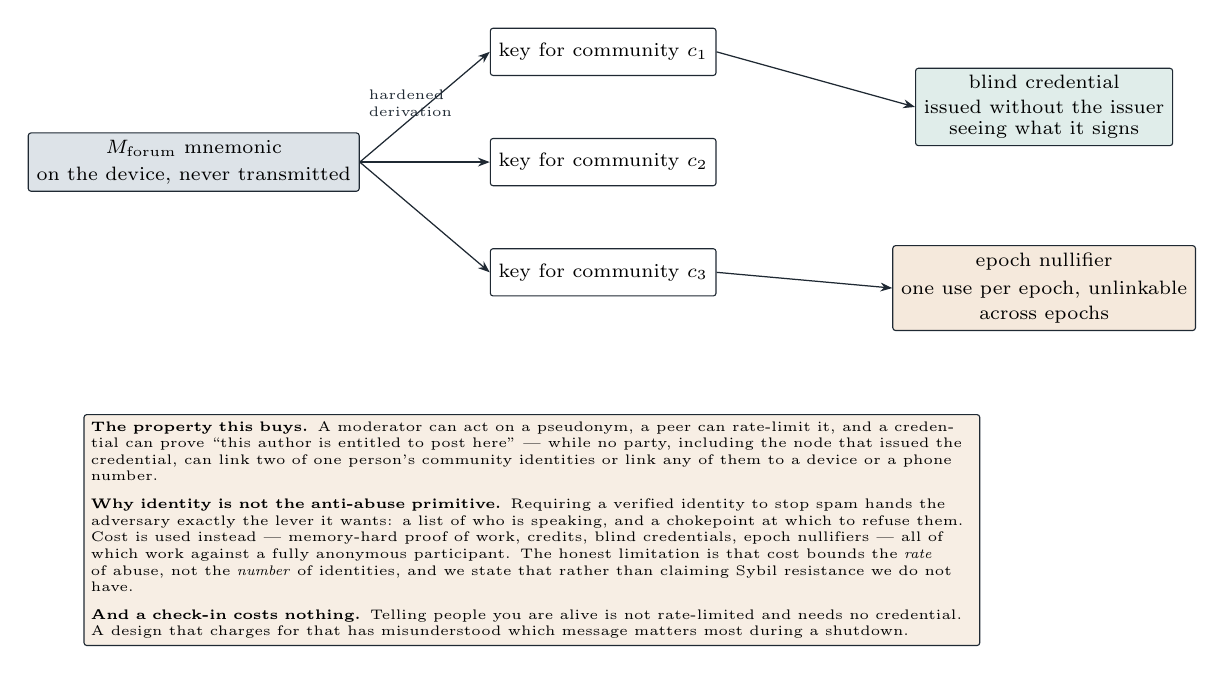
\begin{tikzpicture}[font=\scriptsize]
\node[box,fill=jbMist,minimum width=30mm,minimum height=7mm] (seed) at (0,0)
  {\shortstack{$M_{\text{forum}}$ mnemonic\\[1pt]\scriptsize on the device, never transmitted}};
\node[box,fill=white,minimum width=26mm,minimum height=6mm] (k1) at (5.2,1.4)  {key for community $c_1$};
\node[box,fill=white,minimum width=26mm,minimum height=6mm] (k2) at (5.2,0)    {key for community $c_2$};
\node[box,fill=white,minimum width=26mm,minimum height=6mm] (k3) at (5.2,-1.4) {key for community $c_3$};
\foreach \k in {k1,k2,k3} { \draw[flow] (seed.east) -- (\k.west); }
\node[slbl,anchor=west,align=left] at (2.1,0.75) {hardened\\derivation};

\node[box,fill=jbTeal!16,minimum width=32mm,minimum height=9mm] (cred) at (10.8,0.7)
  {\shortstack{blind credential\\[1pt]\scriptsize issued without the issuer\\\scriptsize seeing what it signs}};
\node[box,fill=jbAmber!18,minimum width=32mm,minimum height=9mm] (null) at (10.8,-1.6)
  {\shortstack{epoch nullifier\\[1pt]\scriptsize one use per epoch, unlinkable\\\scriptsize across epochs}};
\draw[flow] (k1.east) -- (cred.west);
\draw[flow] (k3.east) -- (null.west);

\node[note,anchor=north west,text width=112mm] at (-1.4,-3.2)
{\textbf{The property this buys.} A moderator can act on a pseudonym, a peer can rate-limit it, and a
credential can prove ``this author is entitled to post here'' — while no party, including the node
that issued the credential, can link two of one person's community identities or link any of them to a
device or a phone number.\\[4pt]
\textbf{Why identity is not the anti-abuse primitive.} Requiring a verified identity to stop spam
hands the adversary exactly the lever it wants: a list of who is speaking, and a chokepoint at which
to refuse them. Cost is used instead — memory-hard proof of work, credits, blind credentials, epoch
nullifiers — all of which work against a fully anonymous participant. The honest limitation is that
cost bounds the \emph{rate} of abuse, not the \emph{number} of identities, and we state that rather
than claiming Sybil resistance we do not have.\\[4pt]
\textbf{And a check-in costs nothing.} Telling people you are alive is not rate-limited and needs no
credential. A design that charges for that has misunderstood which message matters most during a
shutdown.};
\end{tikzpicture}
%% ---- END FIGURE J ---------------------------------------------------------

\clearpage
%% ===========================================================================
\figtitle{Figure K — Threat model on one axis: what is resisted, and what is not}
{A compact version of §5 for reviewers who read figures first. The left column is
gated in the implementation; the right column is deliberately unbought.}

%% ---- BEGIN FIGURE K -------------------------------------------------------
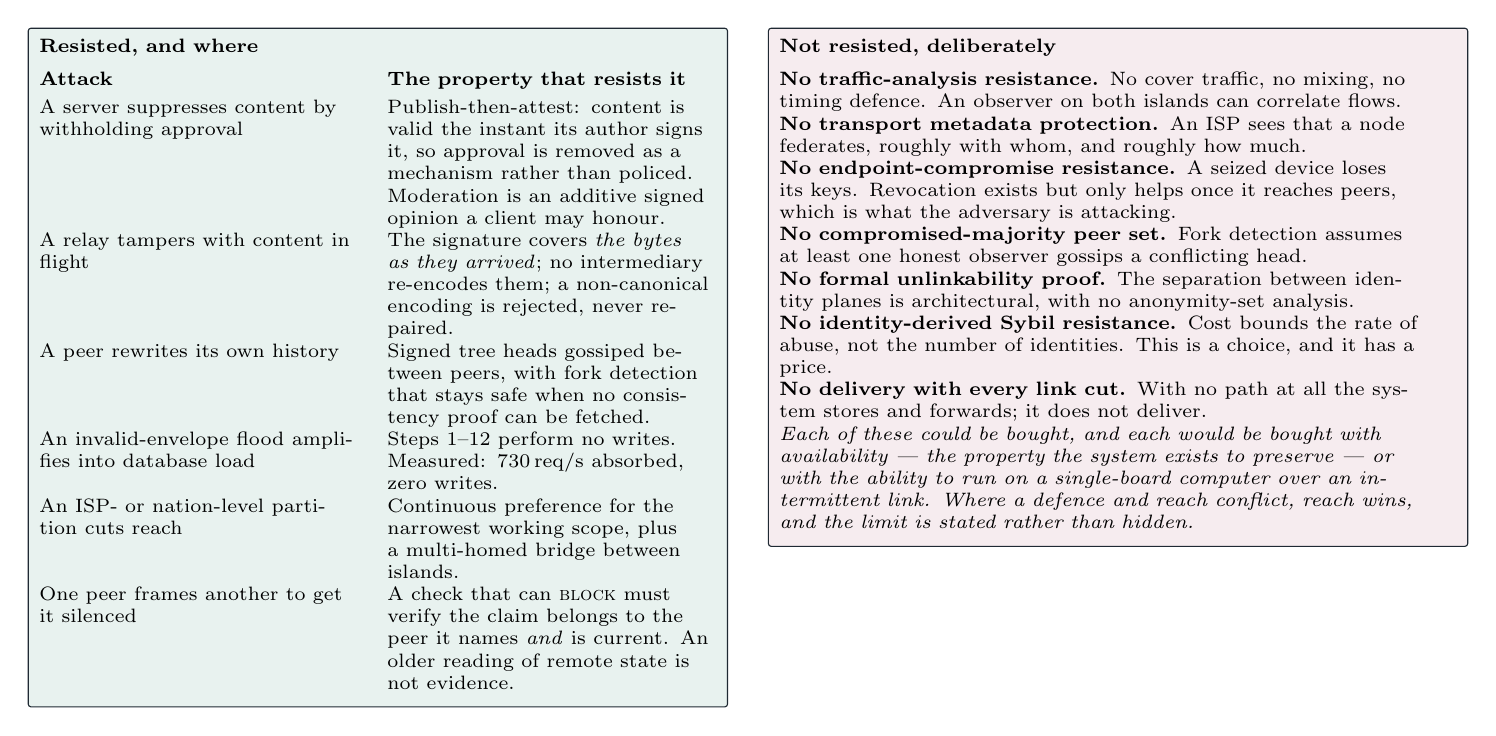
\begin{tikzpicture}[font=\scriptsize]
\node[box,fill=jbTeal!12,text width=86mm,align=left,anchor=north west,inner sep=4pt] (in) at (0,0)
{\textbf{Resisted, and where}\\[4pt]
\begin{tabular}{@{}p{40mm}p{42mm}@{}}
\textbf{Attack} & \textbf{The property that resists it}\\[2pt]
A server suppresses content by withholding approval
 & Publish-then-attest: content is valid the instant its author signs it, so approval is removed as a
   mechanism rather than policed. Moderation is an additive signed opinion a client may honour.\\[3pt]
A relay tampers with content in flight
 & The signature covers \emph{the bytes as they arrived}; no intermediary re-encodes them; a
   non-canonical encoding is rejected, never repaired.\\[3pt]
A peer rewrites its own history
 & Signed tree heads gossiped between peers, with fork detection that stays safe when no consistency
   proof can be fetched.\\[3pt]
An invalid-envelope flood amplifies into database load
 & Steps 1--12 perform no writes. Measured: 730\,req/s absorbed, zero writes.\\[3pt]
An ISP- or nation-level partition cuts reach
 & Continuous preference for the narrowest working scope, plus a multi-homed bridge between islands.\\[3pt]
One peer frames another to get it silenced
 & A check that can \textsc{block} must verify the claim belongs to the peer it names \emph{and} is
   current. An older reading of remote state is not evidence.\\
\end{tabular}};

\node[box,fill=jbRose!10,text width=86mm,align=left,anchor=north west,inner sep=4pt] at (9.4,0)
{\textbf{Not resisted, deliberately}\\[4pt]
\begin{tabular}{@{}p{82mm}@{}}
\textbf{No traffic-analysis resistance.} No cover traffic, no mixing, no timing defence. An observer on
both islands can correlate flows.\\[3pt]
\textbf{No transport metadata protection.} An ISP sees that a node federates, roughly with whom, and
roughly how much.\\[3pt]
\textbf{No endpoint-compromise resistance.} A seized device loses its keys. Revocation exists but only
helps once it reaches peers, which is what the adversary is attacking.\\[3pt]
\textbf{No compromised-majority peer set.} Fork detection assumes at least one honest observer gossips
a conflicting head.\\[3pt]
\textbf{No formal unlinkability proof.} The separation between identity planes is architectural, with
no anonymity-set analysis.\\[3pt]
\textbf{No identity-derived Sybil resistance.} Cost bounds the rate of abuse, not the number of
identities. This is a choice, and it has a price.\\[3pt]
\textbf{No delivery with every link cut.} With no path at all the system stores and forwards; it does
not deliver.\\[6pt]
\emph{Each of these could be bought, and each would be bought with availability — the property the
system exists to preserve — or with the ability to run on a single-board computer over an intermittent
link. Where a defence and reach conflict, reach wins, and the limit is stated rather than hidden.}\\
\end{tabular}};
\end{tikzpicture}
%% ---- END FIGURE K ---------------------------------------------------------

\clearpage
%% ===========================================================================
\figtitle{Figure L --- Audit-log server workflow: acknowledgement becomes portable evidence}
{The audit-log server does not moderate content or report the node's live state. It independently
checks and preserves proof that a node acknowledged a particular signed request.}

%% ---- BEGIN FIGURE L -------------------------------------------------------
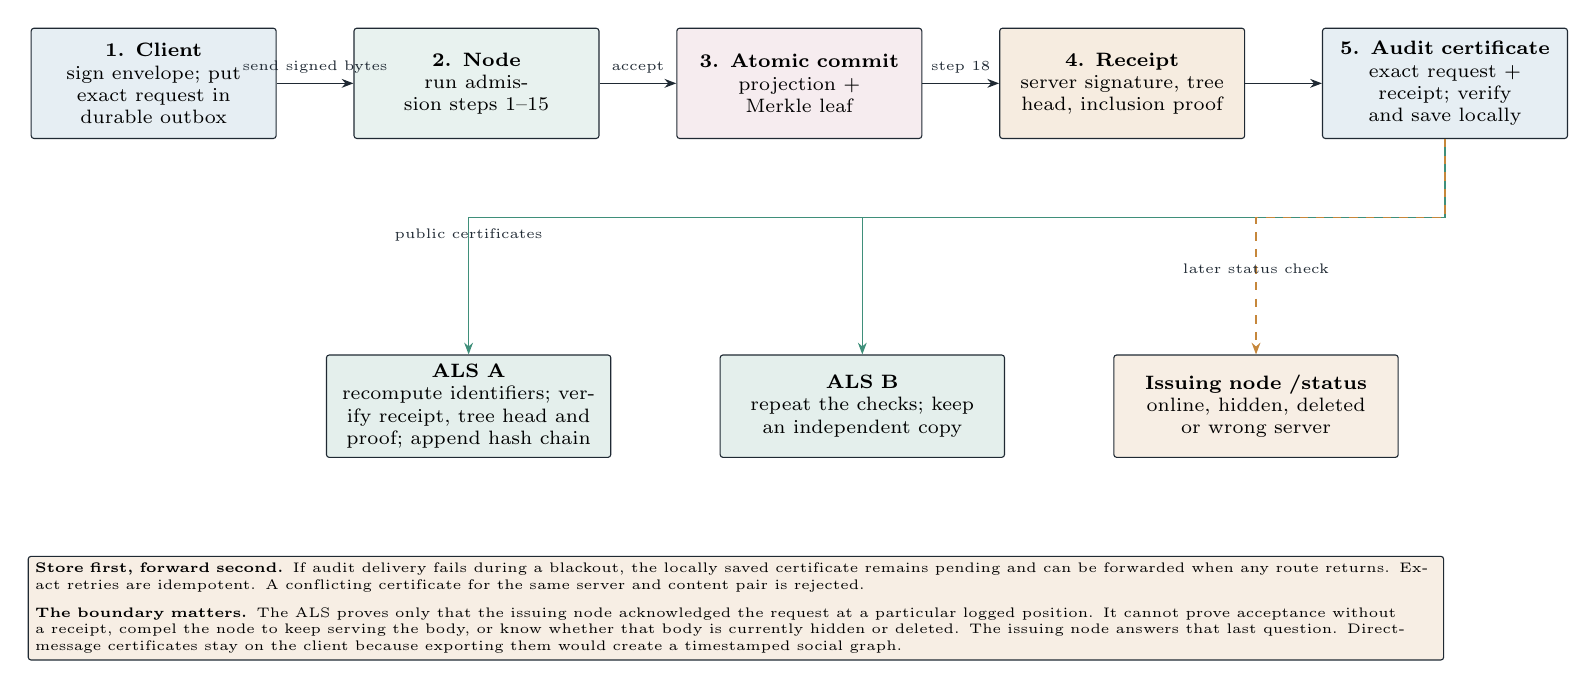
\begin{tikzpicture}[font=\scriptsize,
  stage/.style={box,text width=29mm,minimum height=14mm,align=center,inner sep=3pt},
  audit/.style={box,text width=34mm,minimum height=13mm,align=center,inner sep=3pt}]
\node[stage,fill=jbBlue!12] (client) at (0,0)
  {\textbf{1. Client}\\sign envelope; put exact request in durable outbox};
\node[stage,fill=jbTeal!12] (validate) at (4.1,0)
  {\textbf{2. Node}\\run admission steps 1--15};
\node[stage,fill=jbRose!10] (commit) at (8.2,0)
  {\textbf{3. Atomic commit}\\projection + Merkle leaf};
\node[stage,fill=jbAmber!16] (receipt) at (12.3,0)
  {\textbf{4. Receipt}\\server signature, tree head, inclusion proof};
\node[stage,fill=jbBlue!12] (cert) at (16.4,0)
  {\textbf{5. Audit certificate}\\exact request + receipt; verify and save locally};

\draw[flow] (client) -- node[slbl,above]{send signed bytes} (validate);
\draw[flow] (validate) -- node[slbl,above]{accept} (commit);
\draw[flow] (commit) -- node[slbl,above]{step 18} (receipt);
\draw[flow] (receipt) -- (cert);

\node[audit,fill=jbTeal!14] (alsa) at (4.0,-4.1)
  {\textbf{ALS A}\\recompute identifiers; verify receipt, tree head and proof; append hash chain};
\node[audit,fill=jbTeal!14] (alsb) at (9.0,-4.1)
  {\textbf{ALS B}\\repeat the checks; keep an independent copy};
\node[audit,fill=jbAmber!14] (status) at (14.0,-4.1)
  {\textbf{Issuing node /status}\\online, hidden, deleted or wrong server};

\draw[flow,jbTeal] (cert.south) -- ++(0,-1.0) -| node[slbl,pos=0.62,above]{public certificates} (alsa.north);
\draw[flow,jbTeal] (cert.south) -- ++(0,-1.0) -| (alsb.north);
\draw[flow,jbAmber,dashed] (cert.south) -- ++(0,-1.0) -| node[slbl,pos=0.74,above]{later status check} (status.north);

\node[note,anchor=north west,text width=178mm] at (-1.6,-6.0)
  {\textbf{Store first, forward second.} If audit delivery fails during a blackout, the locally saved
   certificate remains pending and can be forwarded when any route returns. Exact retries are
   idempotent. A conflicting certificate for the same server and content pair is rejected.\\[4pt]
   \textbf{The boundary matters.} The ALS proves only that the issuing node acknowledged the request
   at a particular logged position. It cannot prove acceptance without a receipt, compel the node to
   keep serving the body, or know whether that body is currently hidden or deleted. The issuing node
   answers that last question. Direct-message certificates stay on the client because exporting them
   would create a timestamped social graph.};
\end{tikzpicture}
%% ---- END FIGURE L ---------------------------------------------------------

\end{document}
